\section{Simulation Study}\label{app:simstudy}

This final section presents simulation results evaluating the performance of our proposed estimators in an idealized setting where the outcome model and measurement error models are known. The first subsection outlines our simulation study. The second subsection presents selected results, including the bias, mean-square error, and coverage rates for our proposed estimators and variance estimates. The final subsection provides additional results analyzing the performance of H-SBW and our proposed variance estimator absent measurement error.

\subsection{Study design}

For our simulations we generate populations of $M_1 = 5000$ states, each with $p_s$ CPUMAs, so that we obtain a population of $N_1 = \sum_{s=1}^{M_1} p_s$ CPUMAs. We draw $p_s \stackrel{iid}\sim \lfloor Exp(0.1) + 10\rfloor$ so that the average number of regions per state is approximately 20. We then generate a 3-dimensional covariate vector $X_{sc}$:

\begin{align}\label{eqn:pheccovariates}
\mu_s \stackrel{iid}\sim N(0, \Sigma_S) \\
X_{sc} \mid \mu_s \stackrel{iid}\sim N(\mu_s, \Sigma_V) 
\end{align}

Define $\Sigma_X = \Sigma_Q + \Sigma_S$. Let $\sigma^2_{x, j}$ be the j-th diagonal element of $\Sigma_X$. Across all simulations, we fix this number to be constant and equal to 2 (i.e. $\sigma^2_{x, j} = \sigma^2_x = 2$). We also fix the off-diagonal elements of both $\Sigma_Q$ and $\Sigma_S$ to be equal and so that $Cor(X_j, X_k) = 0.25$. Finally, let $\rho_{x, j}$ denote the within-state correlation of the observations (i.e. $Cor(X_{j, sc}, X_{j, sd})$ for $c \ne d$). We set this value to be equal for all covariates, so that $\rho_{x, j} = \rho_x$, but vary this parameter across simulations.

We then generate outcomes according to the model:

\begin{align*}
Y_{sc} \mid X_{sc} \sim N(X_{1, sc} + X_{2, sc} + X_{3, sc}, \Omega)
\end{align*}
%
where $\Omega$ is a block-diagonal matrix representing the homoskedastic equicorrelation structure outlined below.

\begin{align}
    \label{eqn:phecvariance1}\Omega &= \begin{pmatrix}
    \Omega_1 & 0 & 0 & ... & 0 \\
    0 & \Omega_2 & 0 &  ...  & 0 \\
    & & ...  & & \\
    0 & 0 & 0 &, ..., & \Omega_{M_1} 
    \end{pmatrix} \\
    \label{eqn:phecvariance2}\Omega_s &= \begin{pmatrix}
    \sigma^2_{\epsilon} + \sigma^2_{\varepsilon} & \sigma^2_{\varepsilon} & \sigma^2_{\varepsilon} & ... & \sigma^2_{\varepsilon} \\
    \sigma^2_{\varepsilon} & \sigma^2_{\epsilon} + \sigma^2_{\varepsilon} & \sigma^2_{\varepsilon}& ... & \sigma^2_{\epsilon} \\
    & & ... & & \\
    \sigma^2_{\varepsilon} & \sigma^2_{\varepsilon} & \sigma^2_{\varepsilon} & ... & \sigma^2_{\epsilon} + \sigma^2_{\varepsilon}
    \end{pmatrix}
\end{align}
%
In other words $\sigma^2_{\varepsilon}$ represents the variance component from a state-level random effect and $\sigma^2_{\epsilon}$ represents a variance component from a CPUMA-level random effect, as described in the main paper.

We next generate our noisy outcome and covariate estimates $(J, W)$:

\begin{align*}
(J_{sc}, W_{sc}) \mid (Y_{sc}, X_{sc}) \stackrel{iid}\sim N((Y_{sc}, X_{sc}), \Sigma_{\nu, sc})
\end{align*}

\begin{align*}
    \Sigma_{\nu, sc} = \begin{pmatrix}
    \sigma^2_{\nu, sc} & 0 & 0 & 0 \\
    0 & \sigma^2_{\nu, sc} & 0 & 0 \\
    0 & 0 & \sigma^2_{\nu, sc} & 0 \\
    0 & 0 & 0 & \sigma^2_{\nu, sc}
    \end{pmatrix}
\end{align*}

We allow $\sigma^2_{\nu, sc}$ to either be constant or a function of the sample size of an underlying survey that generates the estimate. In the latter case we simulate these sample sizes $r_{sc} \stackrel{iid}\sim Unif(300, 2300)$. We then generate $\sigma_{\nu, sc}^2$ from the common variance model assumed in the ``heterogeneous adjustment:''

\begin{align*}
    \sqrt{r_{sc}}\sigma^2_{\nu, sc} \stackrel{iid}\sim N(0, \sigma^2_{\nu}^\star)
\end{align*}
%
where $\sigma_{\nu}^{2\star}$ represents the common variance under this model. We then define $\sigma_{\nu}^2$ as

\begin{align*}
    \sigma_{\nu}^2 =
     \sigma_\nu^{2\star}\mathbb{E}[1/r_{sc}]
\end{align*}
%
Given $\sigma_{\nu}^2$, we then define the parameter $\tau$:

\begin{align*}
    \tau = \sigma^2_x/(\sigma^2_x + \sigma^2_{\nu})
\end{align*}

We consider different values of $\tau$ throughout our simulations. This parameter reflects the extent of the measurement error, with $\tau = 1$ meaning that the covariates are measured without error, and the noise increasing as $\tau$ goes to zero.

Define $\rho^\star = \sigma^2_{\varepsilon}/(\sigma^2_{\epsilon} + \sigma^2_{\varepsilon} + \sigma^2_{\nu})$. $\rho^\star$ represents the within-state correlation of the outcome model errors given the true covariates $X$, including the measurement errors in the outcome. We fix this to be 0.25 for our primary simulation results. We caveat that $\rho^\star$ only represents an optimal value in a setting without measurement error. This is due to the contribution of additional terms in the variance of the estimator from the noisy covariate measurements.  

We then consider all 18 combinations of the following parameters:

\begin{itemize}
    \item $r_{sc} \stackrel{iid}\sim Unif(300, 2300); r_{sc} = 1$ 
    \item $\rho_x \in \{0, 0.25, 0.5\}$
    \item $\tau \in \{0.85, 0.9, 0.95\}$
\end{itemize}

For each parameterization we take 500 random samples of size $m_1 = 25$ states (with $n_1$ total CPUMAs that average around 450). For each sample we estimate a series of H-SBW weights that set $\delta = 0$ and the target $\upsilon_0 = (1, 1, 1)$. Let $\rho$ denote the assumed $\rho^\star$ in the H-SBW objective. We generate weights for all combinations of input datasets $Z$ and correlation-parameters $\rho$:

\begin{itemize}
    \item Z \in \{$W$, $X$, $\hat{X}^{hom}$, $\hat{X}^{hom}$, $\hat{X}^{cor}$\}
    \item $\rho \in \{0, 0.25, 0.5\}$
\end{itemize}

We estimate the variance for each estimator using the leave-one-state-out jackknife, described in Section~\ref{sec:methods}. 

Note: for $\hat{\kappa}$ we use the empirical covariance matrix of $W$, the estimated means $\bar{W}$, and $\hat{\Sigma}_{\nu, sc}$, where we draw $\hat{\Sigma}_{\nu, sc}$ from $\Sigma_{\nu, sc} + N(0, 0.001*450*I_d)$. In other words, when averaged together we assume that $\hat{\Sigma}_{\nu}$ have a fairly precise estimate of $\Sigma_{\nu}$.

\subsection{Selected results}\label{ssec:resultsI}

We present the results where the ``heterogeneous adjustment'' model is correct. The results for the homoskedastic measurement errors are quite similar and we observe in the text where they differ. Figure~\ref{fig:simbias} displays the bias associated with each estimator. From left to right the panels reflect different values of $\tau$: the left-most panels have the most measurement error while the right-most panels have the least. From top to bottom the panels reflect different values of $\rho_x$: the top-most panel has no correlation structure among the covariates, while the bottom-most panels are more highly correlated within state. Within each panel we organize the results by the input covariate set: $W$ represents the estimators generated without any covariate adjustment; $X$ reflects estimators generated on the true covariates; ``Xhat-het'' represents the heterogeneous adjustment ($\hat{X}^{het}$), ``Xhat-hom'' represents the homogeneous adjustment ($\hat{X}^{hom}$), and ``Xhat-cor'' represents the correlated adjustment ($\hat{X}^{cor}$). The estimators are colored by the assumed value of $\rho$ in the H-SBW objective. Across all of the present simulations, we set $\rho^\star$ equal to 0.25.

We highlight two general results. First, if we know the true values of $X$, all of our estimators are unbiased. Second, balancing on $W$ results in bias; moreover, this bias increases as $\tau$ decreases, and increases with $\rho$.  These results are consistent with our propositions in Appendices~\ref{app:AsecI} and ~\ref{app:AsecII}.

When attempting to mitigate this bias by using some estimate of $\mathbb{E}[X \mid W]$, balancing on $\hat{X}^{hom}$, $\hat{X}^{het}$, or $\hat{X}^{cor}$ results in approximately unbiased estimates for all values of $\rho$ when the covariates uncorrelated. When $X$ are correlated across observations, setting $\rho > 0$ results in biased estimates for $\hat{X}^{het}$ or $\hat{X}^{hom}$, where the bias increases with $\rho$. The SBW estimators remain approximately unbiased, even when the data are correlated. We speculate in Remark~\ref{remark:sbwspeculation} why this may be the case. In settings where $\rho_x = 0.25$ the estimators using that $\hat{X}^{cor}$ remain approximately unbiased. However, when $\rho_x = 0.5$ even these estimators appear to have some bias. In further investigations (results available on request), this bias disappears as we increase the number of states. Regardless of the adjustment set, all biases on the adjusted datasets are smaller in absolute magnitude than the corresponding biases associated with estimators that naively balance $W$. 

\begin{figure}[H]
\begin{center}
    \caption{Simulation study: estimator bias}\label{fig:simbias}
    \label{fig:loveplotc1}
    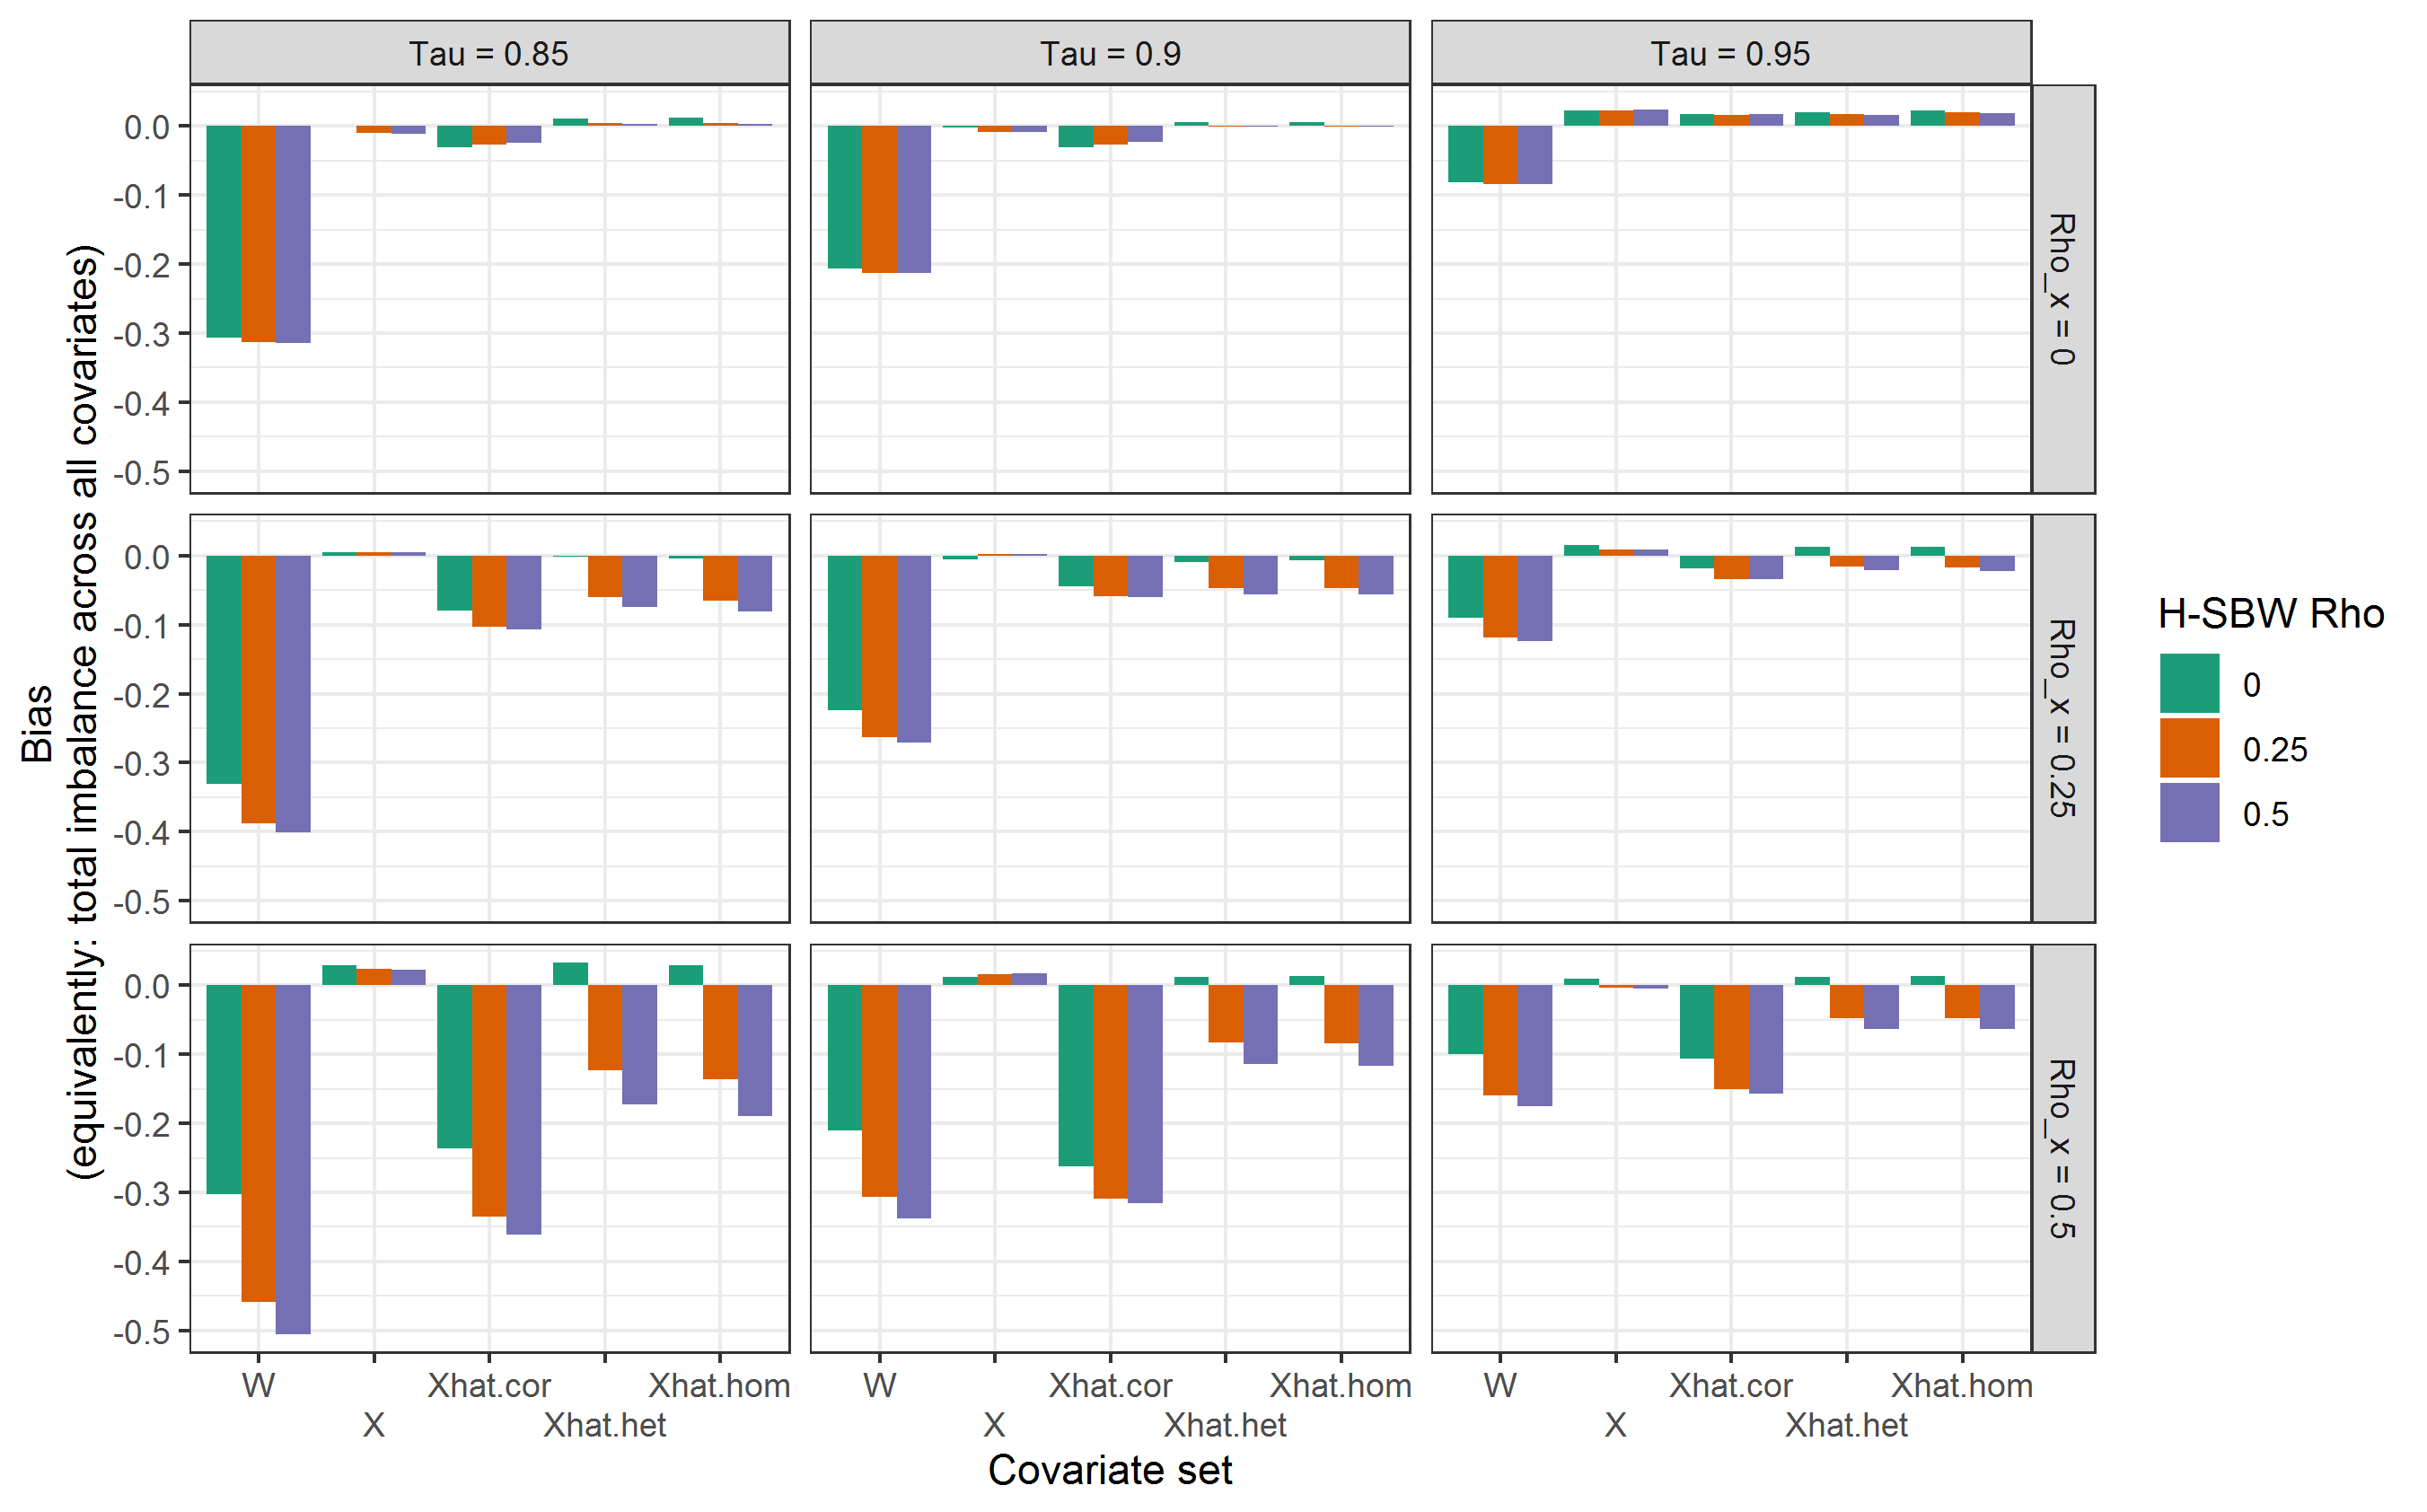
\includegraphics[scale=0.5]{01_Plots/bias-plot.png}
    \subcaption{Averaged across 500 simulations for each specification}
\end{center}
\end{figure}

All of these simulations had heterogeneous measurement error. When examining the results when the errors are homoskedastic we find that the estimators that balance on $\tilde{X}^{het}$ have a small bias even when $\tau = 0$ or $\rho = 0$. Assuming this model is correct when it is not appears to have some cost. This may help explain the slightly worse performance we found when using the heterogeneous adjustment in our validation study in Section~\ref{sec:results}.

Figure~\ref{fig:simvar} displays the variance associated with these same estimators. Throughout we obtain a modest reduction in variance as we increase $\rho$. Choosing either $\rho = 0.25$ or $\rho = 0.5$ gives similar improvements relative to choosing $\rho = 0$. We obtain similar results when considering a wider range of parameterizations of $(\rho, \rho^\star)$ in a context without measurement error (see Section~\ref{appssec:simstudyresults2}).\footnote{In the setting without measurement error $\rho^\star$ represents the optimal value.}

These results also show that balancing on $\hat{X}^{cor}$ can lead to a much more variable estimate, particularly when the covariates have larger within-state correlations. Only in the setting with uncorrelated covariates and little measurement error does the variability induced by this adjustment appears to have less cost.

\begin{figure}[H]
\begin{center}
    \caption{Simulation study: estimator variance}\label{fig:simvar}
    \label{fig:loveplotc1}
    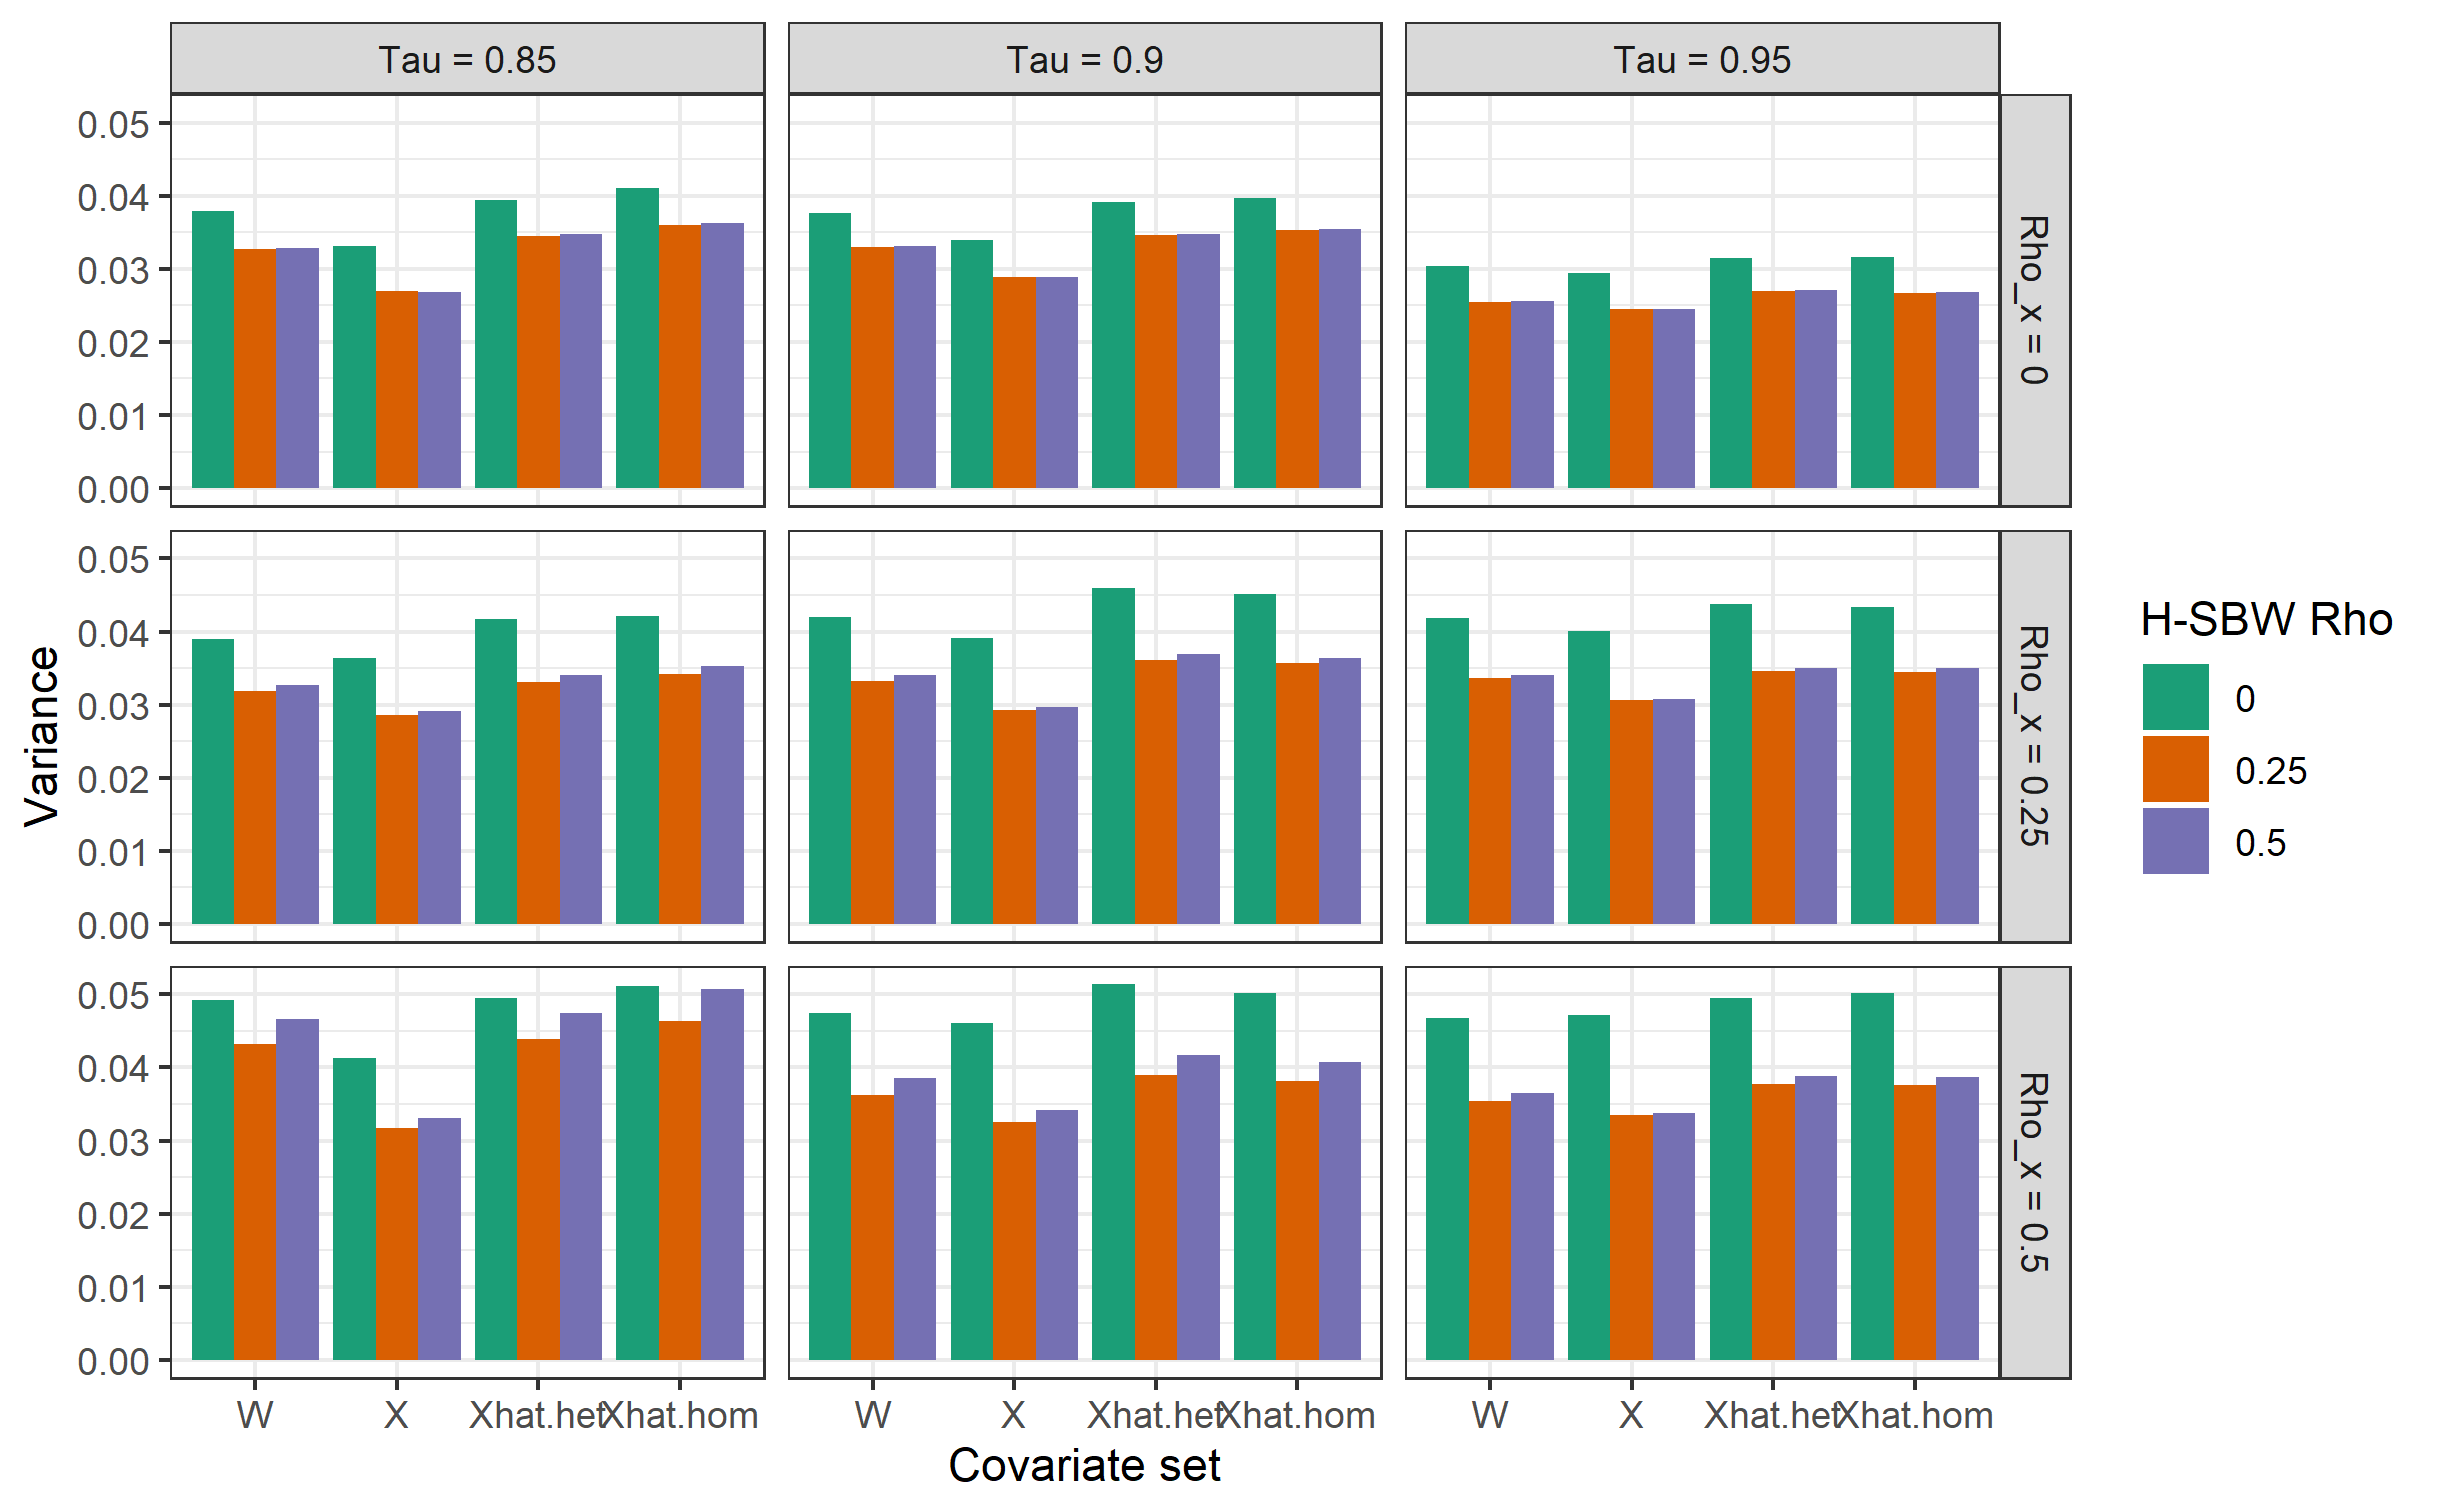
\includegraphics[scale=0.5]{01_Plots/var-plot.png}
    \subcaption{Averaged across 500 simulations for each specification}
\end{center}
\end{figure}

Figure~\ref{fig:simmse} displays the MSE of these estimators. The estimators generated on $\hat{X}^{cor}$ have larger MSE, largely driven by the increase in variability we observed previously. Despite the increase in bias for H-SBW with $\hat{X}^{hom}$ or $\hat{X}^{het}$ we still often find modest MSE reductions when using H-SBW relative to SBW. This appears more likely as the magnitude of the measurement error measurement error decreases and/or the within-state correlation decreases (i.e. moving towards the top-right of the plot). Whether an MSE improvement is possible also depends on $\rho^\star$: if we were to set $\rho^\star = 0$, we would expect the MSE of these estimators to increase for all estimators as $\rho$ increases, even when we observe $X$ (see also Section~\ref{appssec:simstudyresults2}). The results are similar when considering homoskedastic measurement errors, though the space where we see MSE improvements for H-SBW relative to SBW on the uncorrelated adjustments appears to increase slightly (results available on request). 

\begin{figure}[H]
\begin{center}
    \caption{Simulation study: estimator mean-square-error}\label{fig:simmse}
    \label{fig:loveplotc1}
    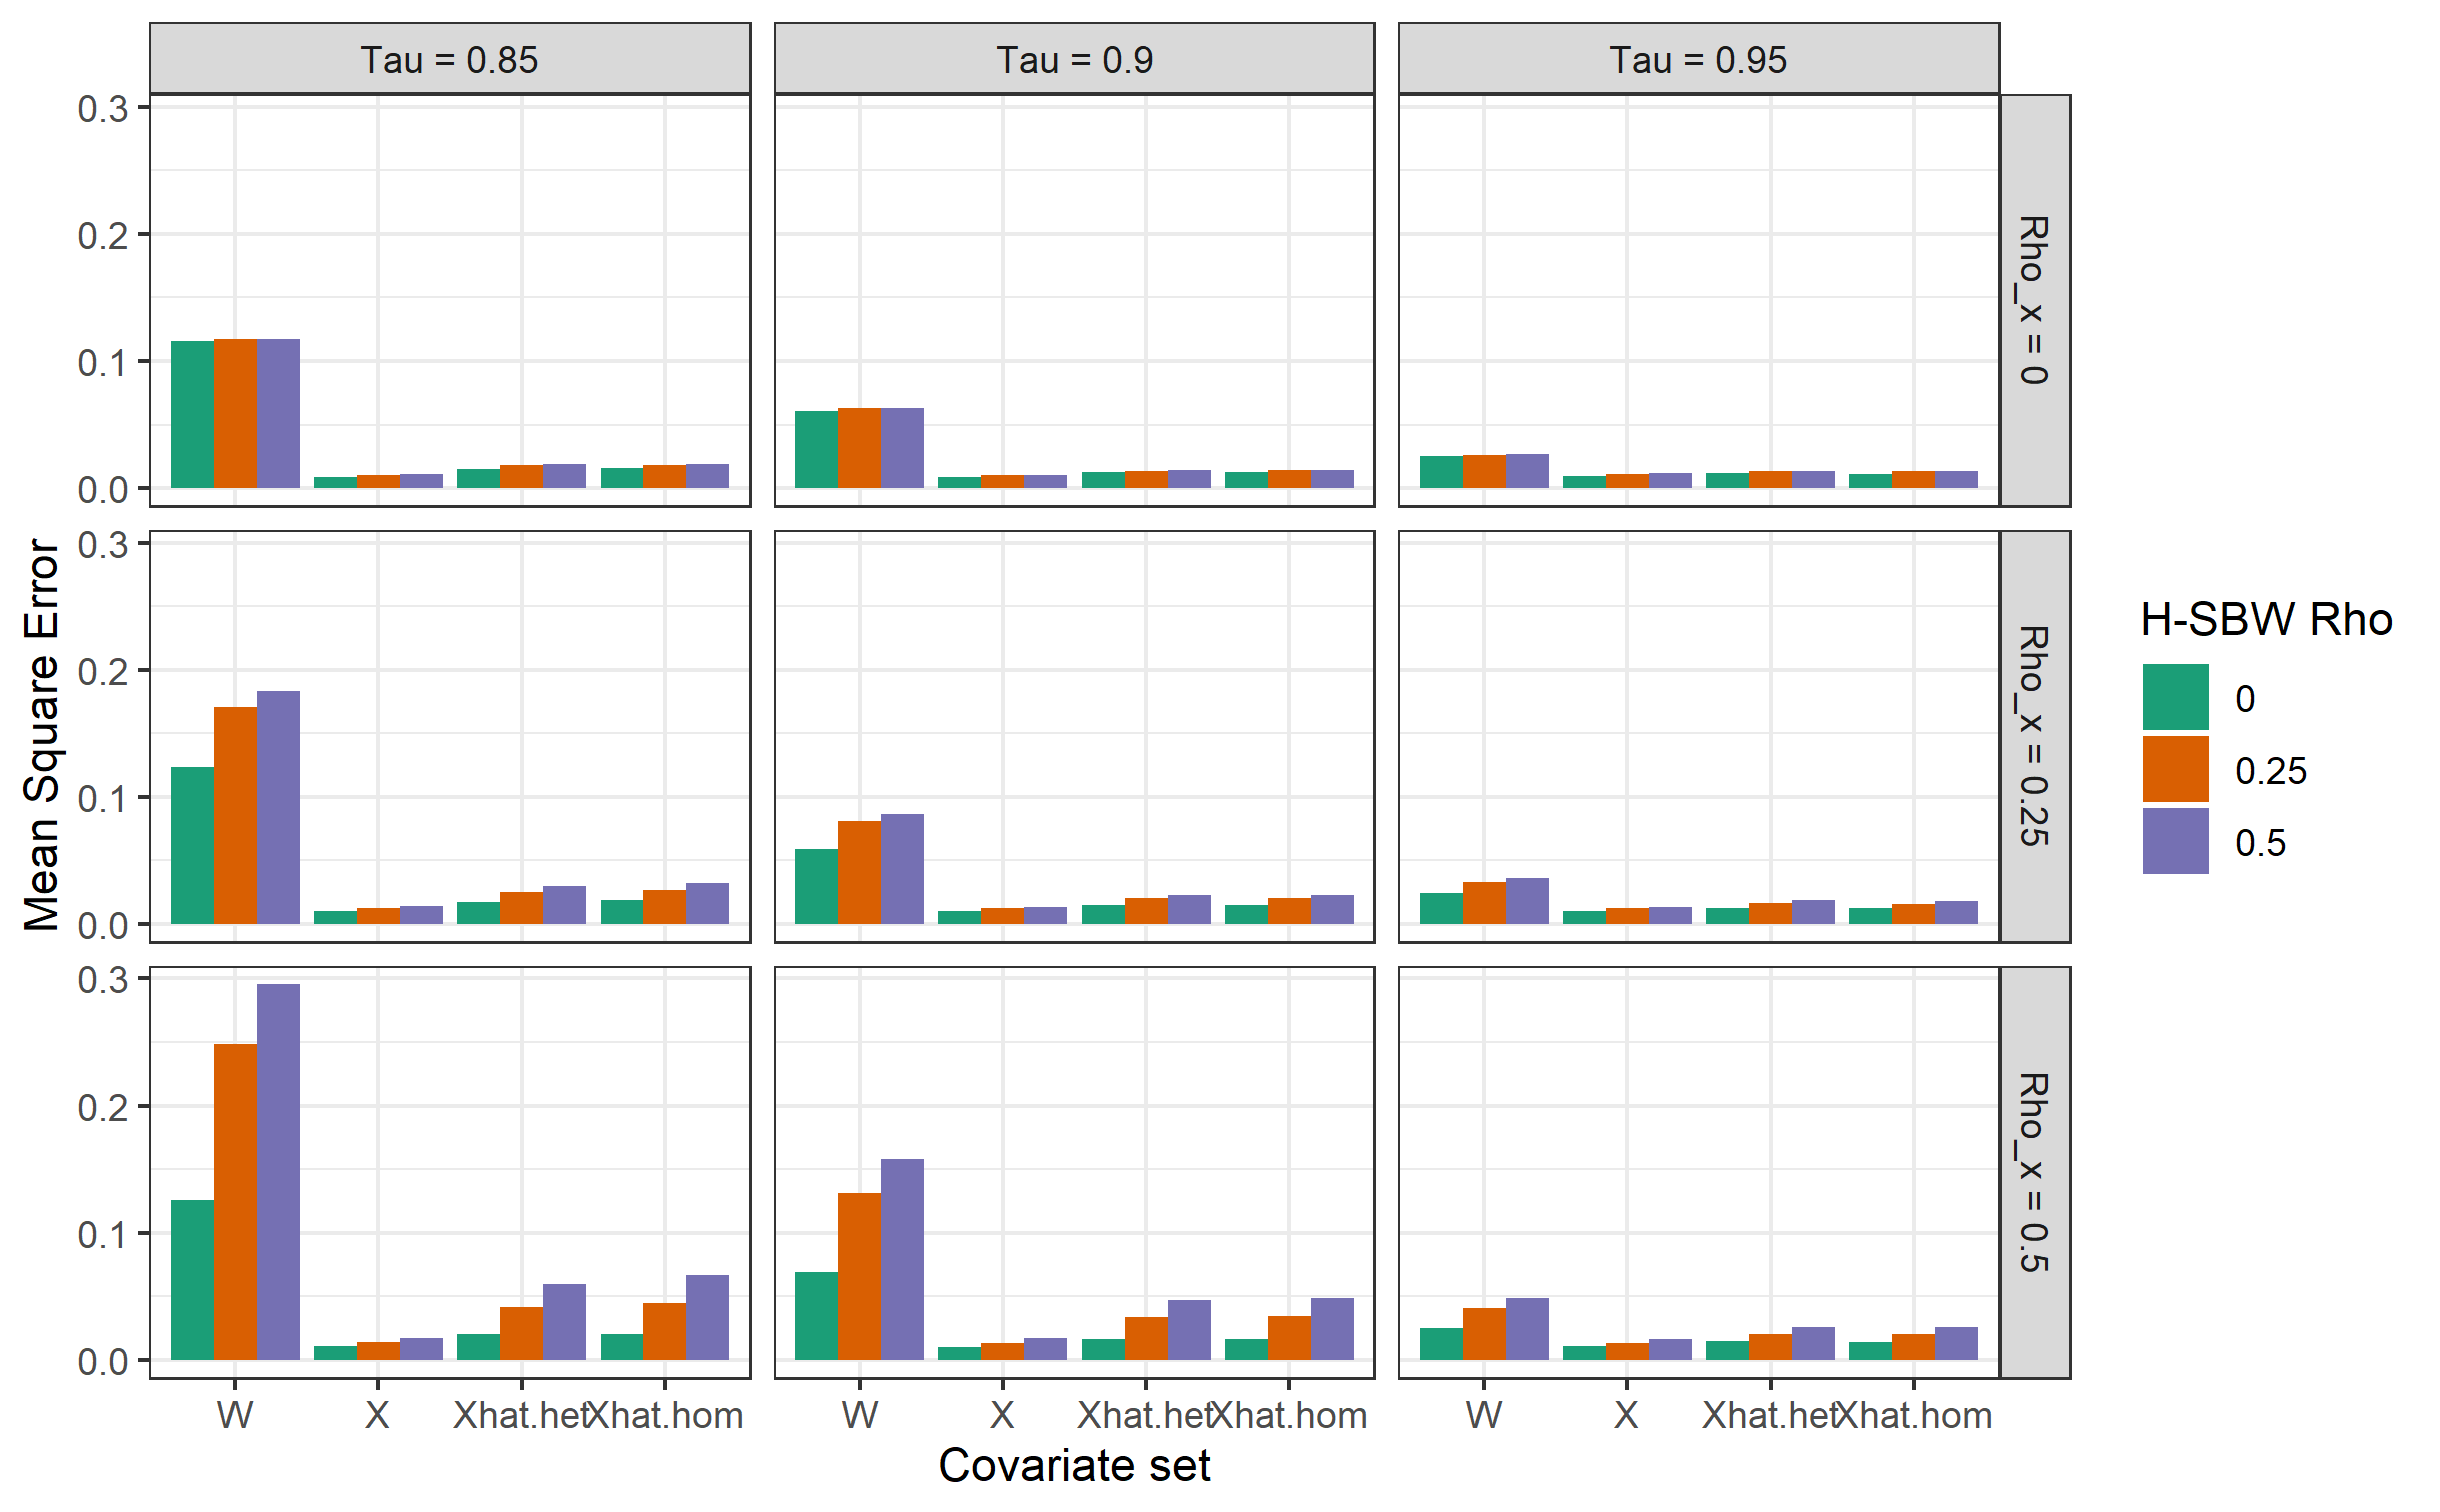
\includegraphics[scale=0.5]{01_Plots/mse-plot.png}
    \subcaption{Averaged across 500 simulations for each specification}
\end{center}
\end{figure}

We next evaluate the performance of the leave-one-state-out jackknife procedure and evaluate confidence interval coverage (for 95\% confidence intervals) and length, and display these results in Figures~\ref{fig:simcoverage1} and ~\ref{fig:simcoverage2}. We use the standard normal quantiles to generate confidence intervals throughout.

Figure~\ref{fig:simcoverage1} shows that when $\rho = 0$ we obtain approximately nominal coverage rates across all specifications that use $X$ or some version of $\hat{X}$. However we fail ever achieve nominal coverage rates when balancing on $W$. Even when the amount of measurement error is small ($\tau = 0.95$) we only obtain at best slightly below 90 percent coverage rates. Confidence interval coverage appears to deteriorate as we increase $\rho_x$, even when balancing on the true covariates $X$.\footnote{This is consistent with results in \cite{cameron2008bootstrap}.} Unsurprisingly the rates worsen for estimators generated on $\hat{X}^{het}$ and $\hat{X}^{hom}$ in the settings where we found the highest bias. We also obtain slightly less than desired rates for estimators using $X$. This is likely because we do not use any degrees-of-freedom adjustment for our confidence intervals (we examine this further in Section~\ref{appssec:simstudyresults2}). On the other hand, coverage rates are quite conservative for estimators generated on $\hat{X}^{cor}$. The positive bias of the jackknife variance estimates are especially large for this estimator which largely drives this result.\footnote{We almost always find a positive or negligible bias for the unscaled jackknife variance estimates, consistent with Proposition~\ref{prop:jackknife}.}

\begin{figure}[H]
\begin{center}
    \caption{Simulation study: jackknife coverage rates}\label{fig:simcoverage1}
    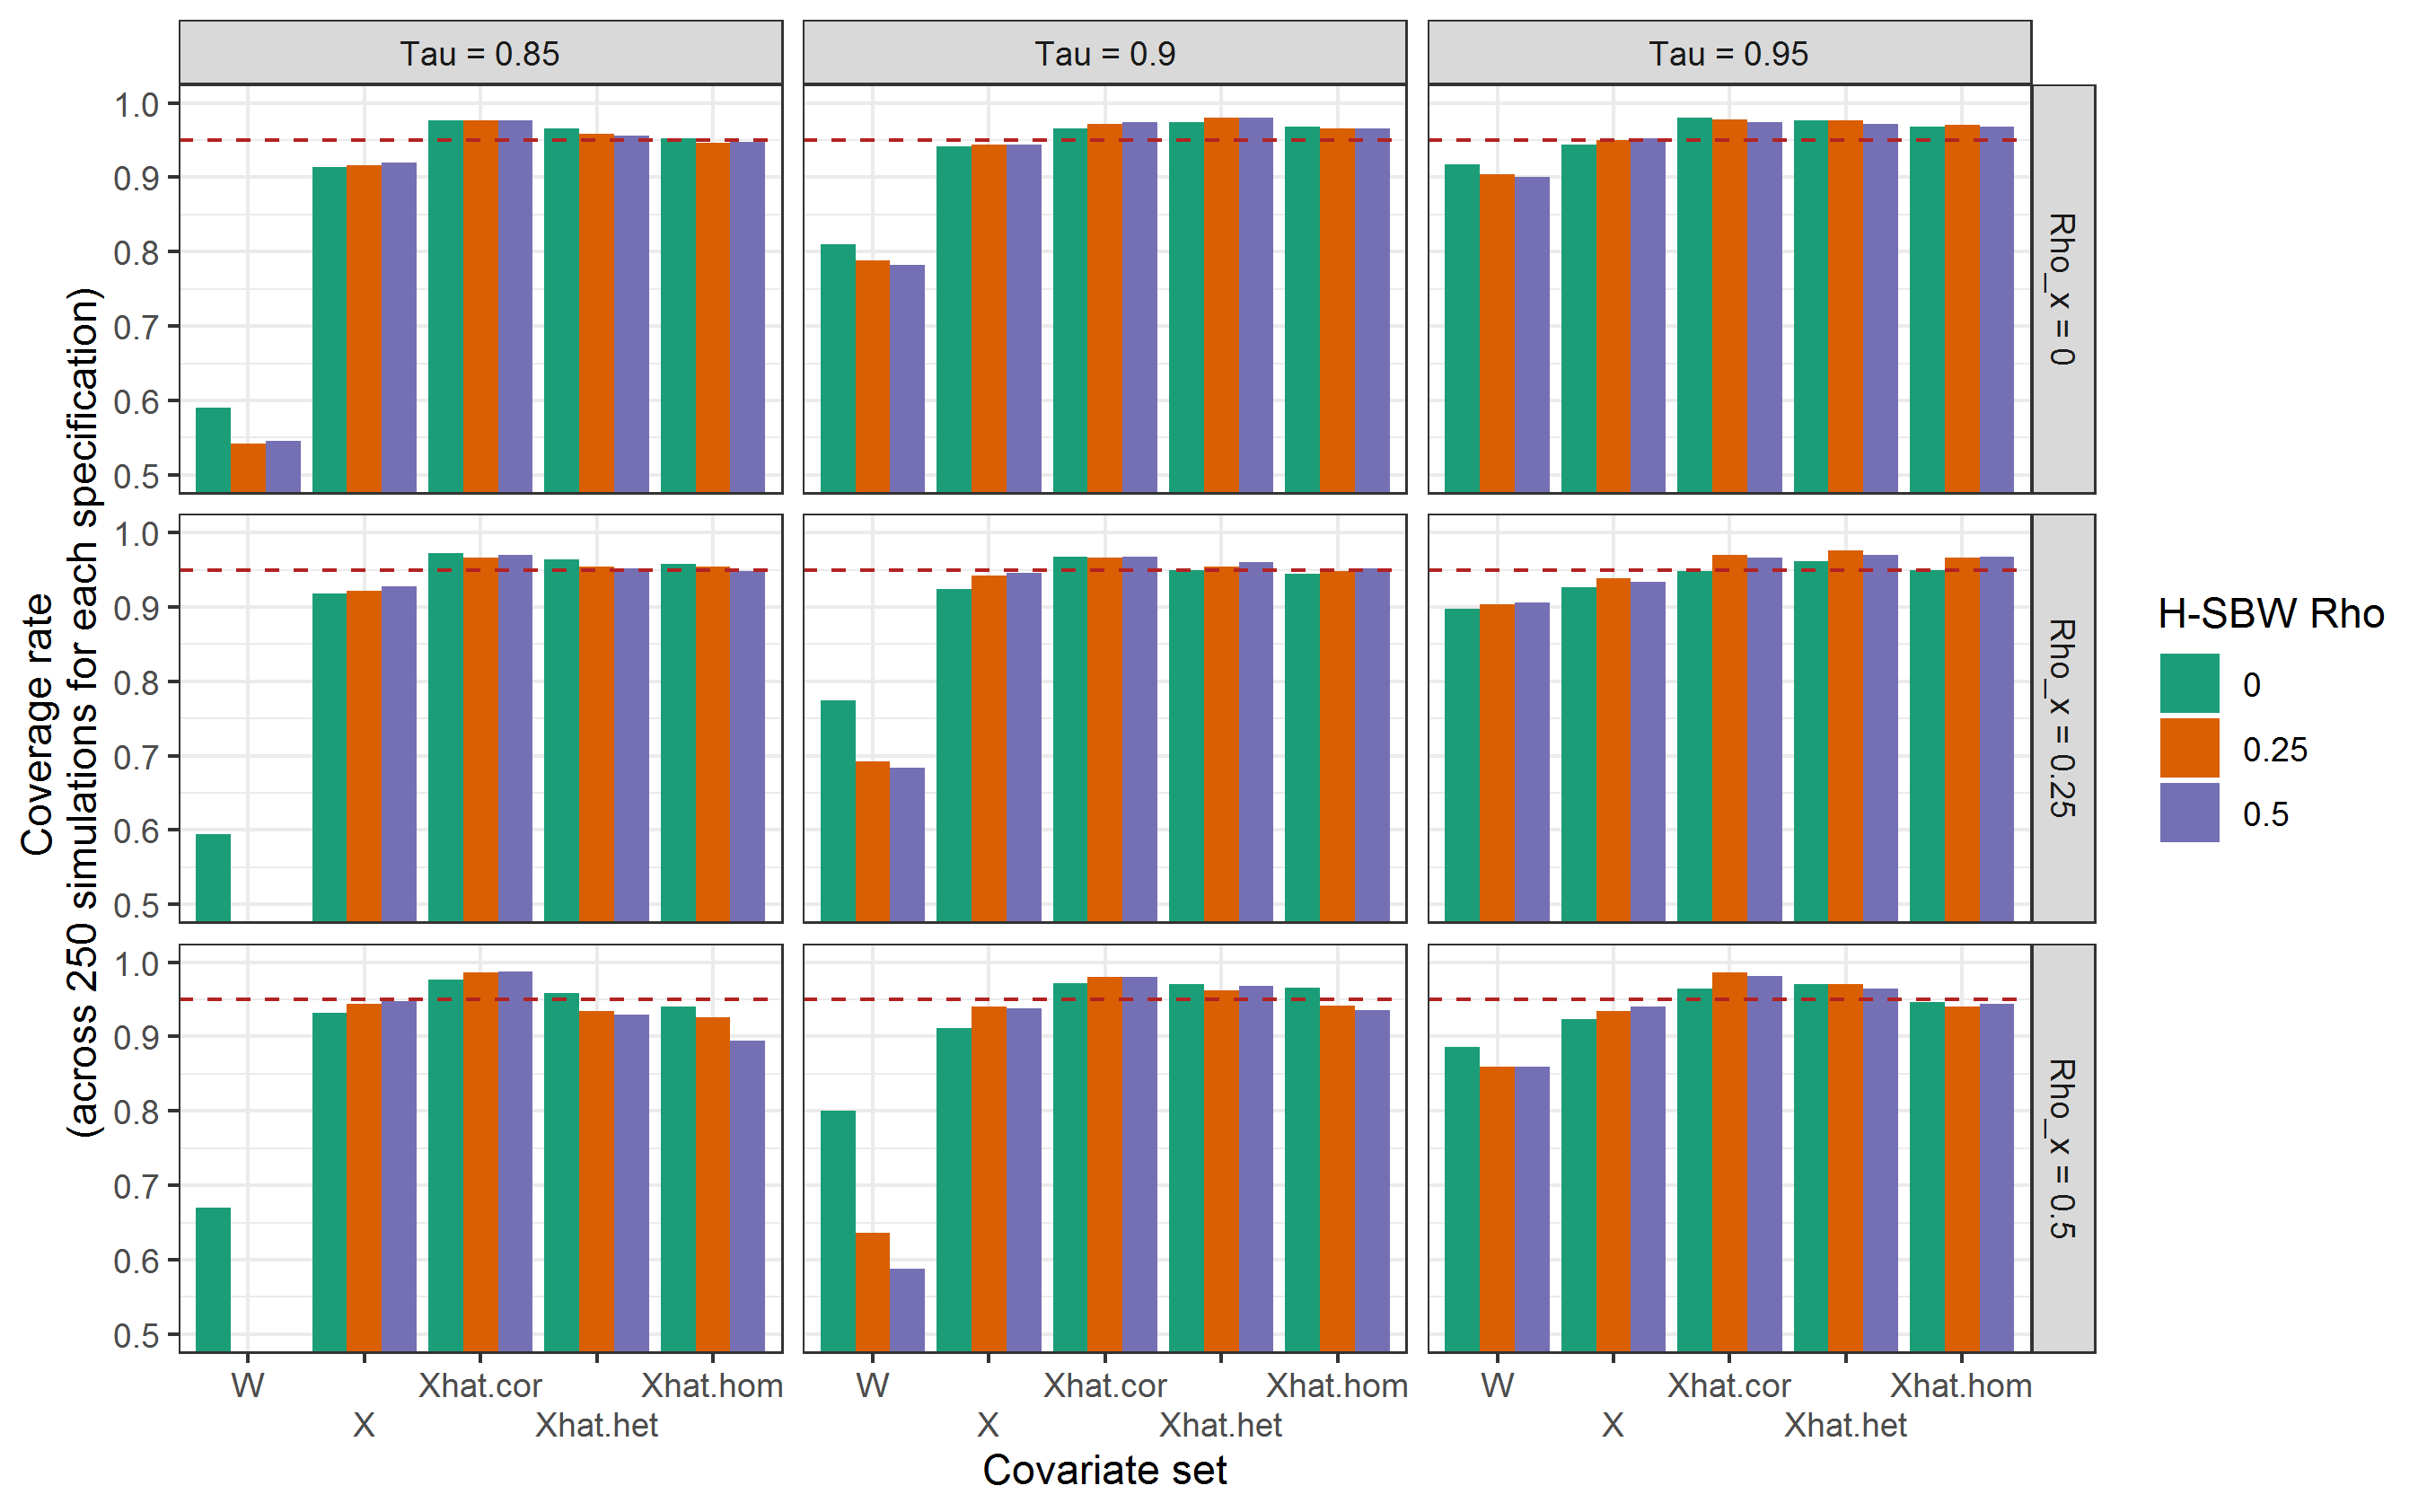
\includegraphics[scale=0.5]{01_Plots/coverage-plot-1.png}
    \subcaption{Averaged across 500 simulations for each specification}
\end{center}
\end{figure}

Figure~\ref{fig:simcoverage2} compares the mean confidence interval lengths using the leave-one-state-out jackknife. The H-SBW estimator is associated with slightly more precise estimates, reflecting that the estimators have decreased variability under our assumed correlation structures. We again see that even when we choose $\rho$ sub-optimally we obtain more precise inferences than when using SBW. This suggests benefits to using H-SBW even when our estimate of $\rho$ is a guess. As the previous results would suggest, we find that the confidence intervals using $\hat{X}^{cor}$ are quite large. The results are similar when considering homoskedastic measurement errors. 

\begin{figure}[H]
\begin{center}
    \caption{Confidence interval length}\label{fig:simcoverage2}
    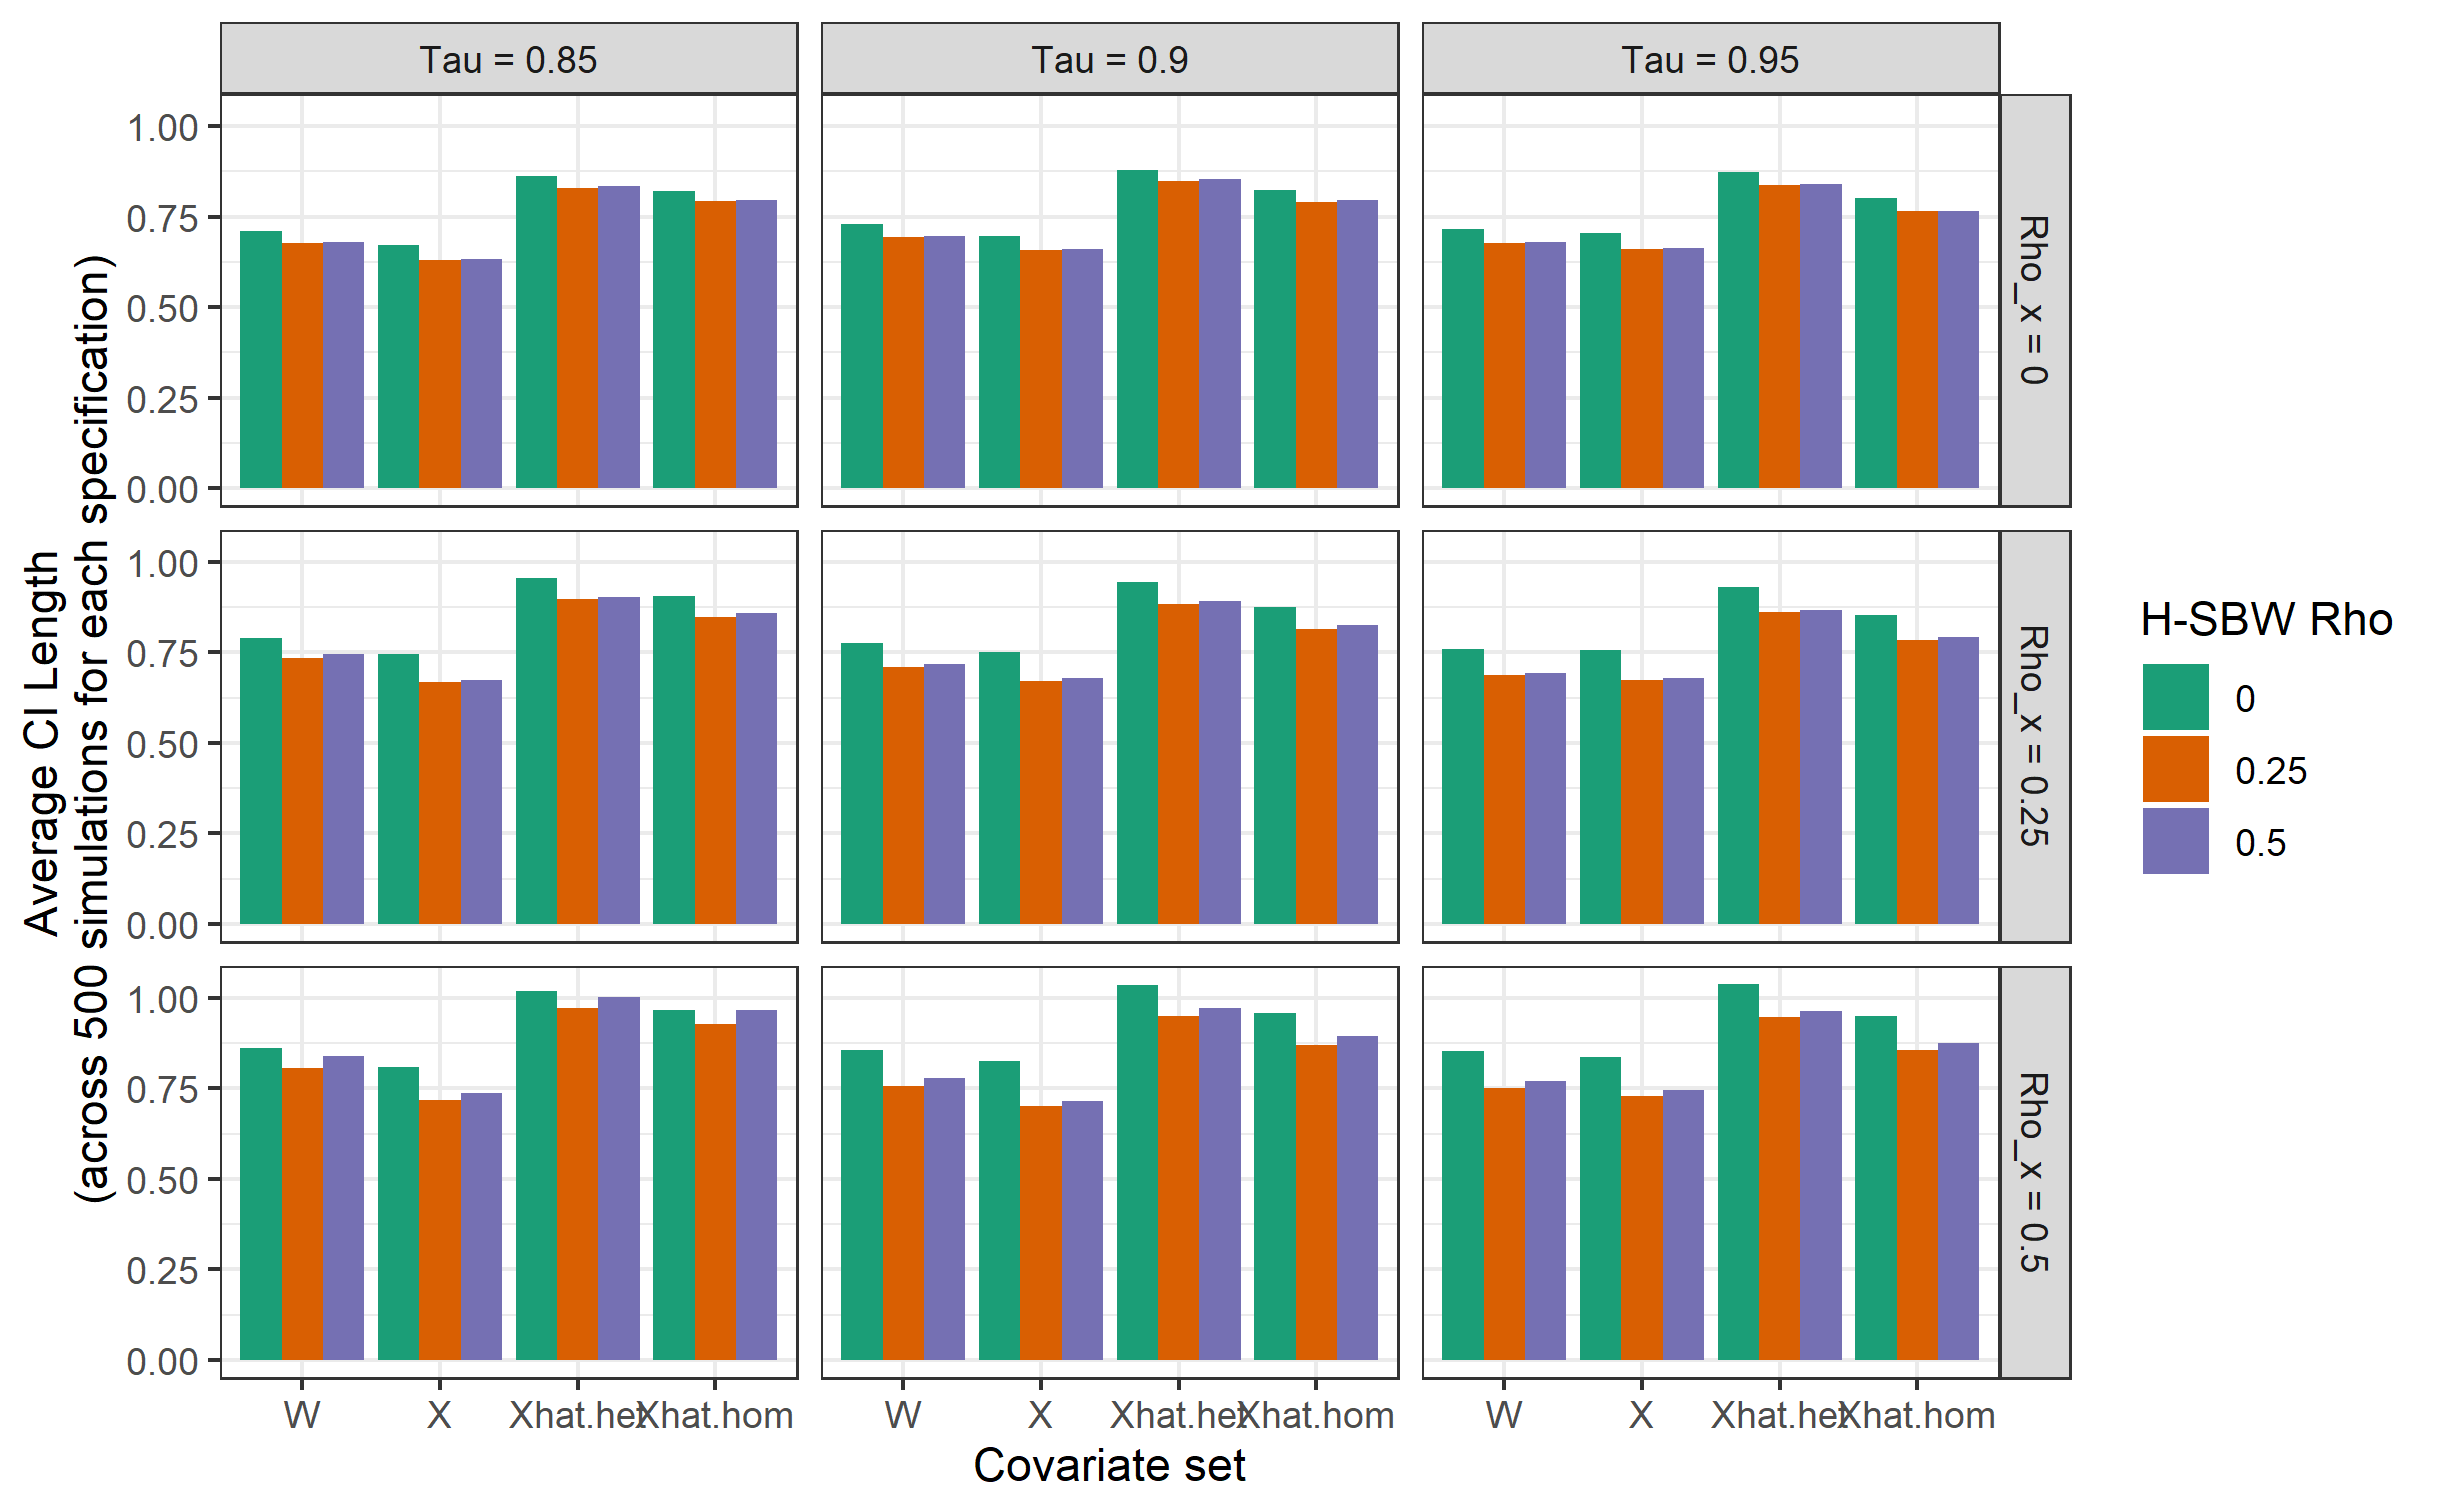
\includegraphics[scale=0.5]{01_Plots/ci-length-plot.png}
    \subcaption{Averaged across 500 simulations for each specification}
\end{center}
\end{figure}

We emphasize four takeaways from this simulation study. First, setting $\rho > 0$ can increase the bias of our proposed estimators in the context of measurement error and dependent data. However, the bias is generally small relative to the bias of balancing on the noisy covariate measurements $W$, and MSE improvements using H-SBW are still possible relative to SBW with the simple covariate adjustments ($\hat{X}^{hom}$ or $\hat{X}^{het}$). Second, despite the improved theoretic properties, accounting for the correlation in the data when using H-SBW (i.e. balancing on $\hat{X}^{cor}$ and the data are measured with error may not be worth the cost in variance given the sample of states we consider here. Third, we find no evidence that the ``heterogeneous adjustment'' improves our subsequent estimates even in an ideal setting. This adjustment may even induce bias when the model is incorrect.\footnote{This finding may in part reflect the distribution of sample sizes we generated, which we took to be uniform. Perhaps with a different distribution these results would differ.} Finally, confidence interval coverage when using the leave-one-state-out jackknife variance estimates give close to nominal coverage rates for our unbiased estimators -- even when using the standard normal quantiles in a setting with 25 states. 

This simulation study assumes throughout that we know the true data generating model for the outcome and that are data are gaussian. Because in practice we would not have such knowledge, this study complements our validation study in Section~\ref{sec:results}, which has more direct bearing on understanding how these estimators might perform in an applied setting.

\subsection{Additional results: H-SBW without measurement error}\label{appssec:simstudyresults2}

We consider additional simulations for the setting where $X$ is known and the outcome model follows homoskedastic but possibly correlated errors. For these results we only vary $\rho^\star \in \{0, 0.25, 0.5, 0.75, 0.99\}$, and fix $\rho_x = 0.25$ throughout. 

Figure~\ref{fig:hsbwvarx} displays the empirical variance of the H-SBW estimators averaged over 1000 simulations. Each panel reflects different values of $\rho^\star$, while the x-axis throughout displays the assumed value of $\rho$ in the H-SBW objective. The red bars indicate when $\rho$ is optimally selected -- $\rho = \rho^\star$. This selection corresponds with the lowest variance estimator as we expect. Consistent with our previous results, when $\rho^\star > 0$ any assumed $\rho$ improves the variance of the resulting estimator relative to SBW. Of course, this requires in general that our assumed correlation structure of the error terms is correct.

\begin{figure}[H]
\begin{center}
    \caption{Variance of H-SBW estimator for known covariates}\label{fig:hsbwvarx}
    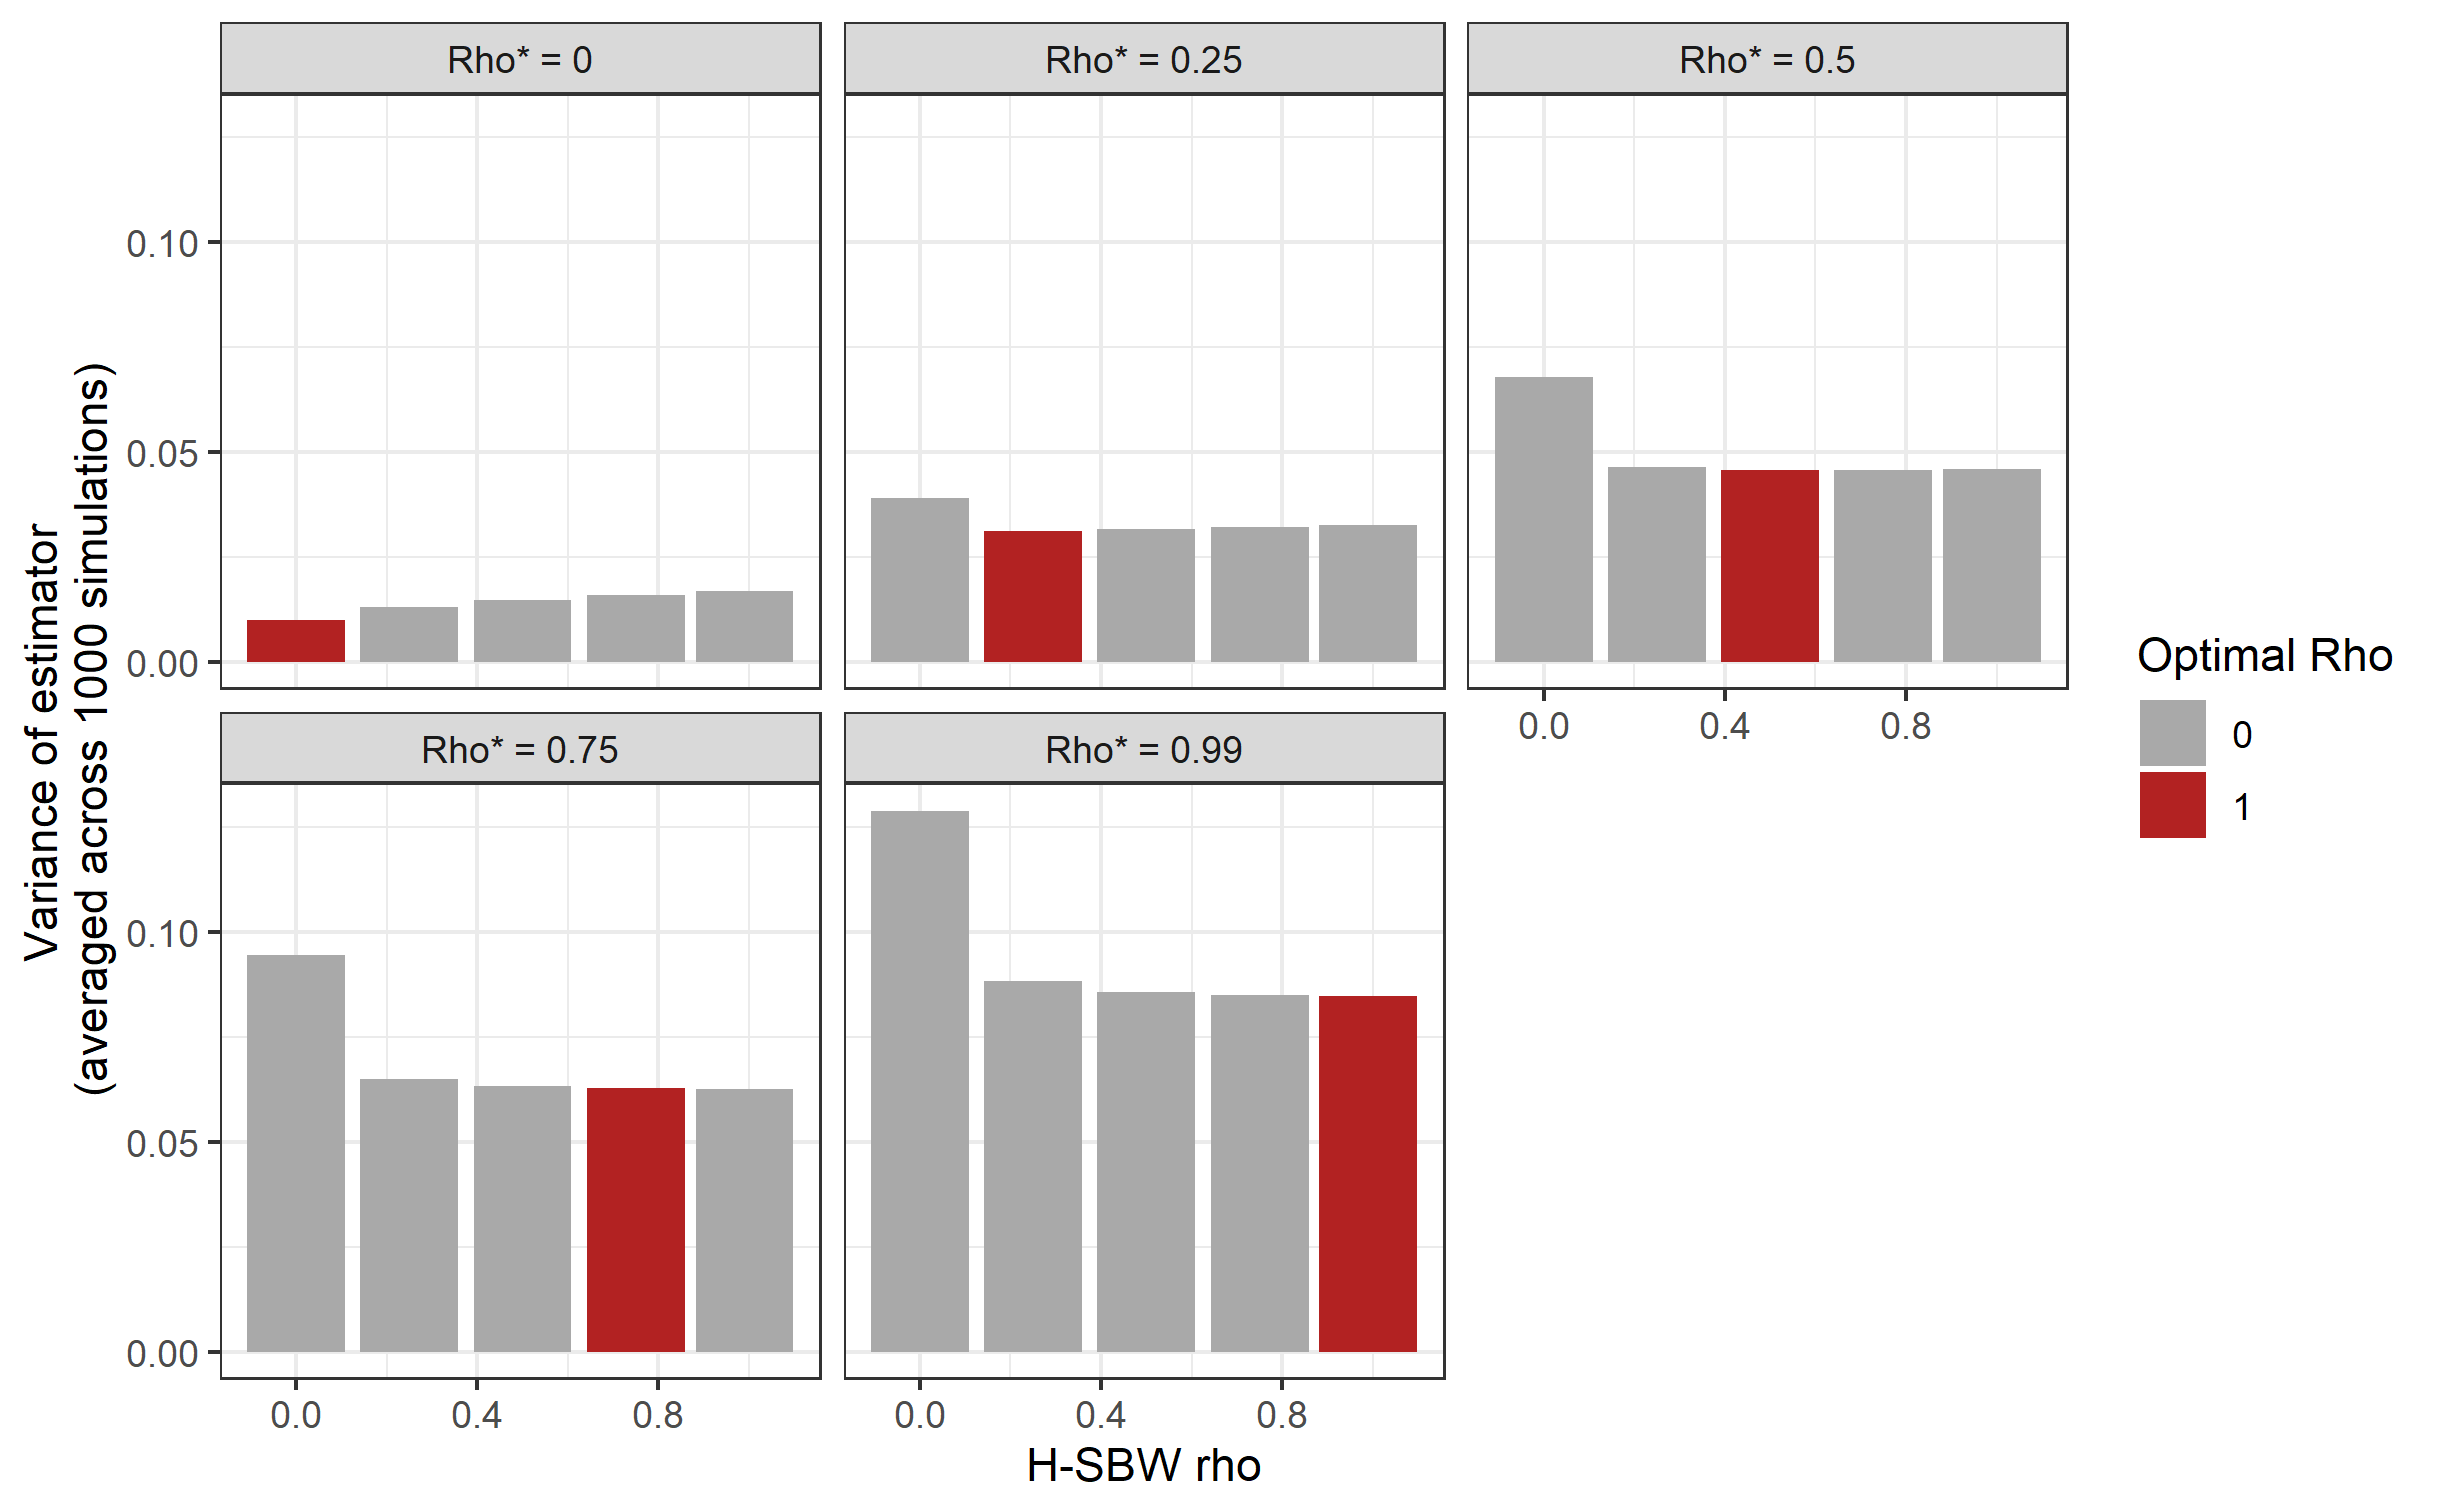
\includegraphics[scale=0.5]{01_Plots/variance-x-plot.png}
    \subcaption{Averaged across 1000 simulations for each specification}
\end{center}
\end{figure}

We conclude by examining the confidence interval coverage for the leave-one-state-out-jackknife. Figure~\ref{fig:hsbwcoveragex} displays the results. Consistent with our previous findings we obtain slightly less than nominal coverage rates, particularly when $\rho^\star$ is small. This slight undercoverage is likely due to our use of standard normal quantiles to generate the confidence intervals.\footnote{Consistent with Proposition~\ref{prop:jackknife} and the previous results we again find that the unscaled variance estimates are all either positively or negligibly biased.} Interestingly, coverage appears to improve when setting $\rho > 0$ even when $\rho^\star = 0$. We speculate that by more evenly dispersing the weights across states, H-SBW may be increasing the effective degrees of freedom of the estimator (see, e.g., \cite{cameron2015practitioner}), illustrating another potential benefit of this approach. Analyzing the theoretic properties of these variances estimators in this setting is beyond the scope of the present study but would provide interesting future work.

\begin{figure}[H]
\begin{center}
    \caption{H-SBW coverage for known covariates}\label{fig:hsbwcoveragex}
    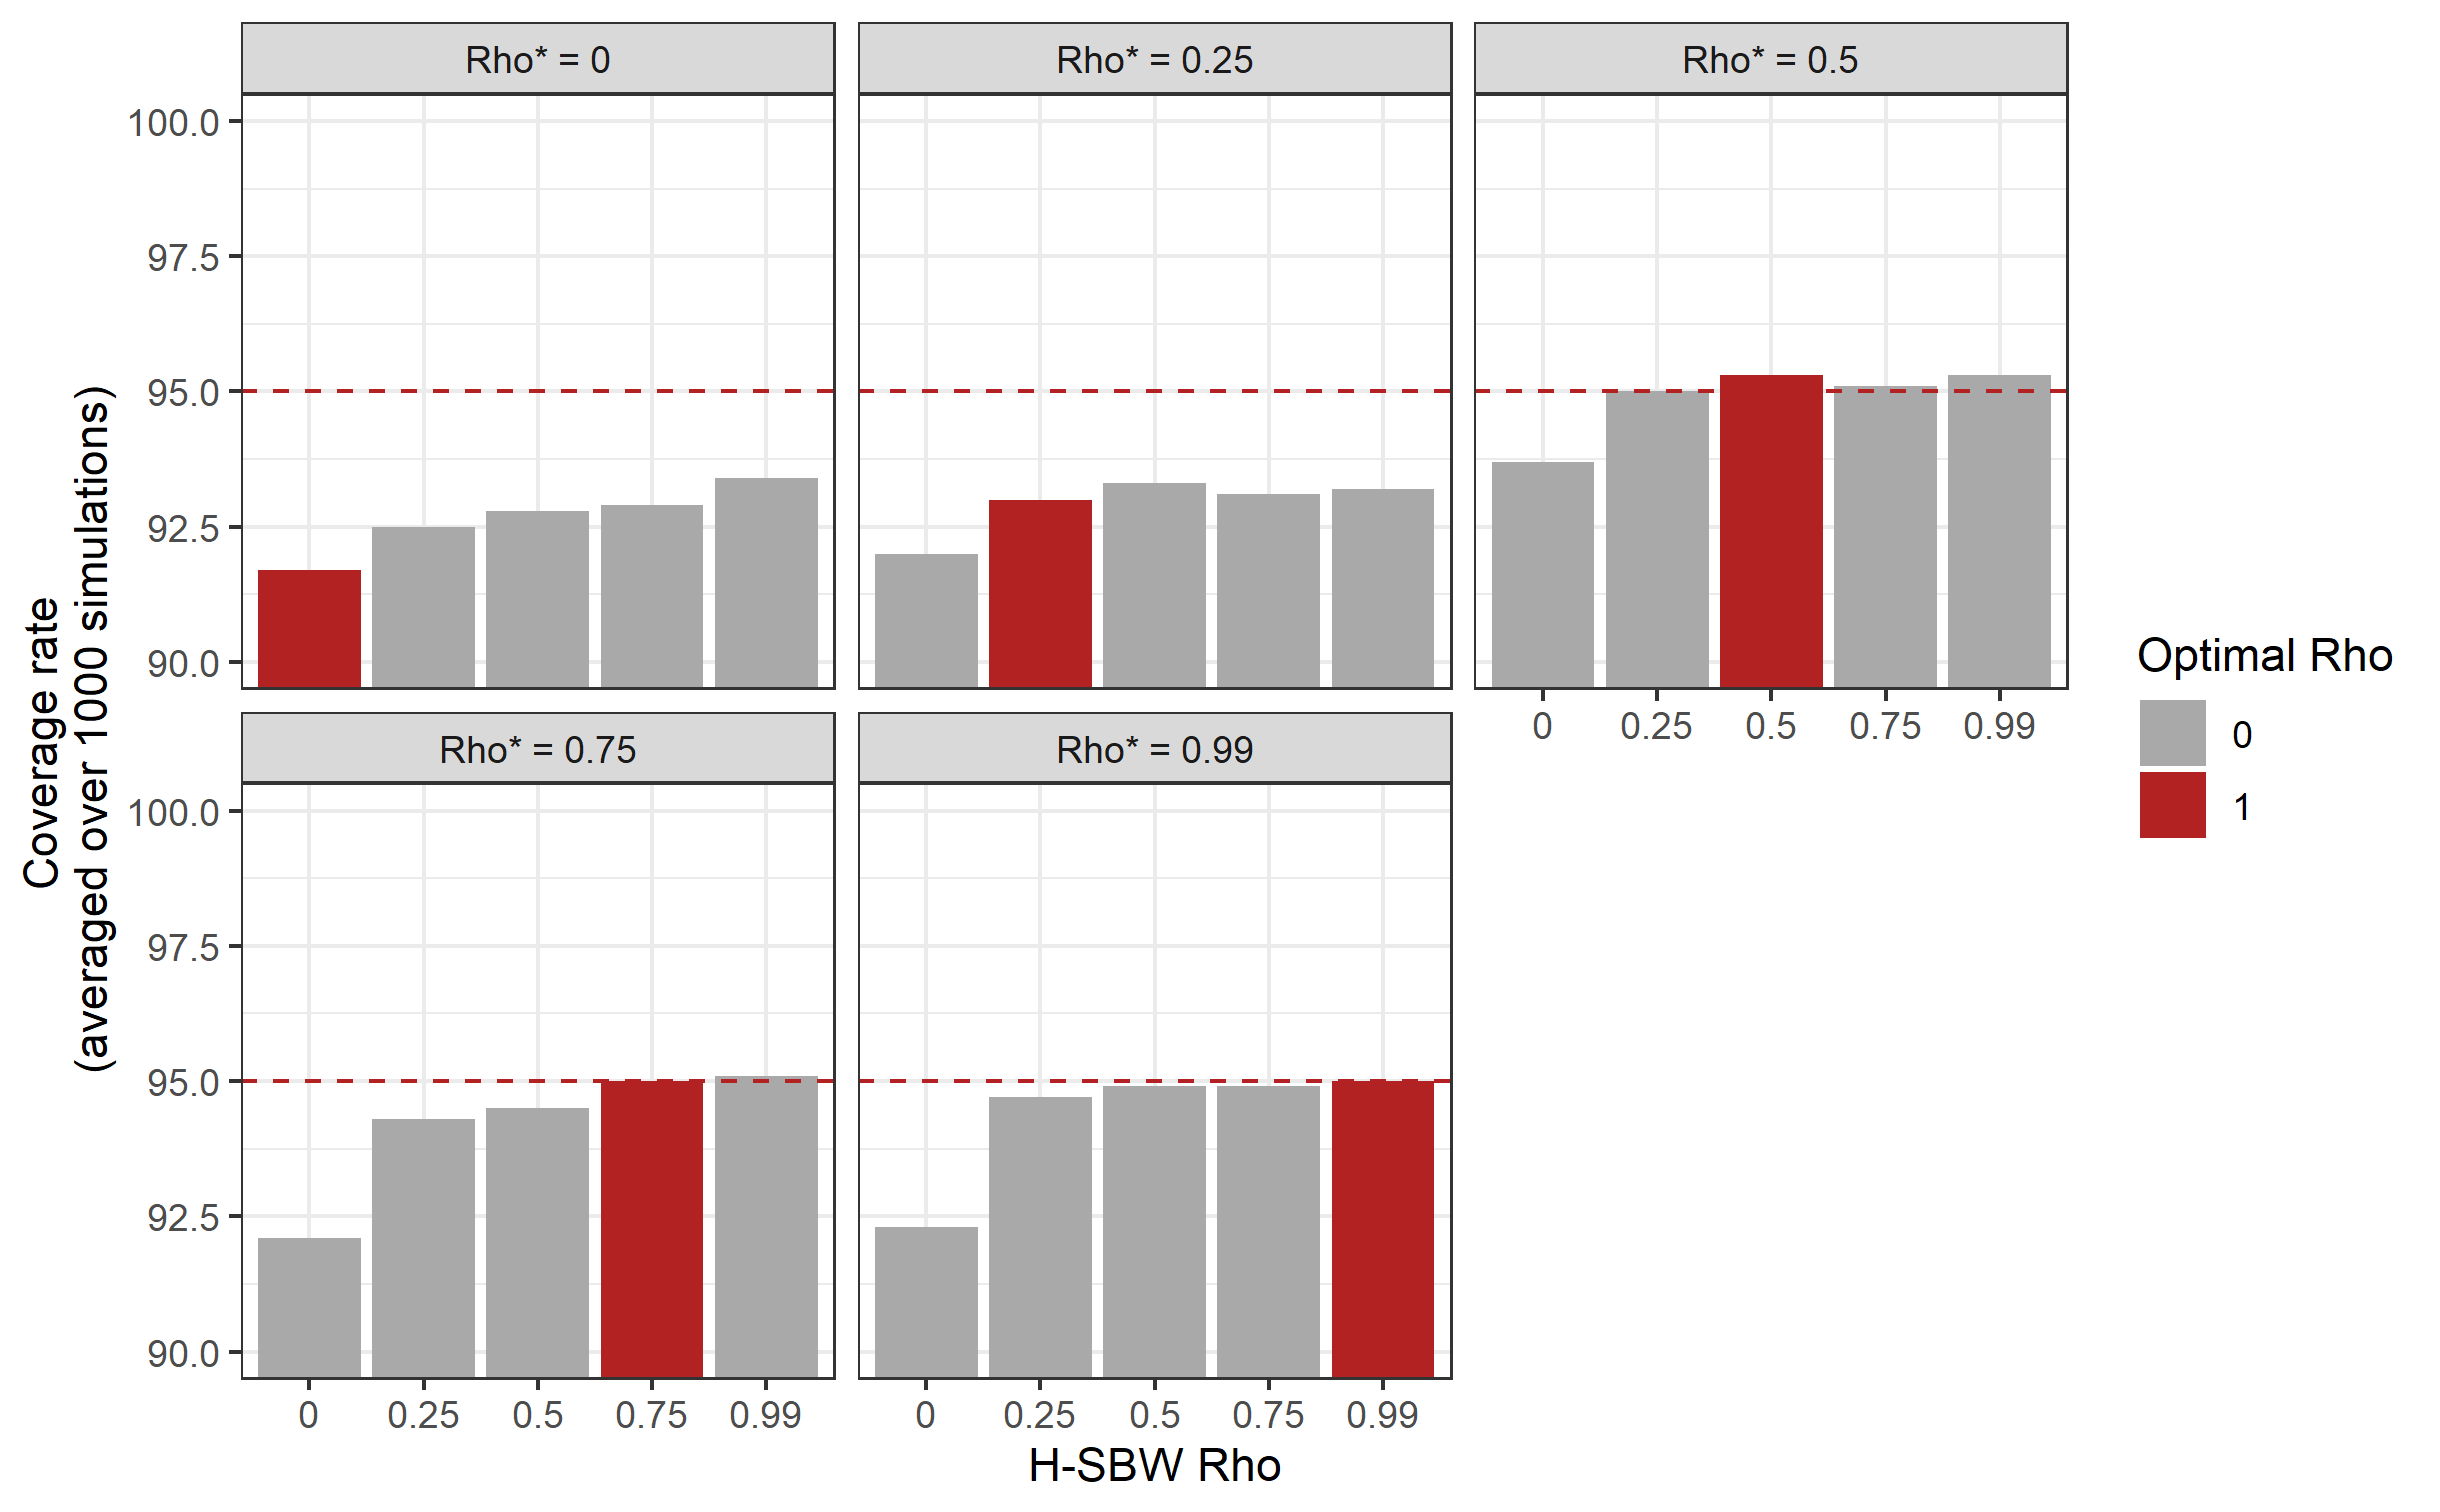
\includegraphics[scale=0.5]{01_Plots/coverage-x-plot.png}
    \subcaption{Averaged across 1000 simulations for each specification}
\end{center}
\end{figure}

